\documentclass[twoside]{report}


%%%%% LANGUE ET ENCODAGE %%%%%
\usepackage[T1]{fontenc}
\usepackage{csquotes} % recommended to ensure that quoted texts are typeset according to the rules of your main language
\usepackage[french]{babel}


%%%%% IMPORT CONFIG %%%%%
%%-----------------------------------------------------------------%%
%%
%%  This page only manages constants linked to the master's work. 
%%
%%-----------------------------------------------------------------%%

% Intitulé du Travail de Master (TM)
\newcommand{\titre}{Titre du Travail de Master}

% Nom de l'auteur du TM
\newcommand{\auteur}{Jules Bolomey}

% Date de fin du TM
\newcommand{\dateTM}{Juillet 1900}  

% Nom de l'orientation du Master 
\newcommand{\orientation}{Ingénierie géomatique}

% Titre et nom du directeur du travail de master
\newcommand{\directeur}{Prof. Dr. Alain Berset}

% Titre et nom du co-directeur s'il existe
\newcommand{\codirecteur}{Prof. Dr. Albert Einstein}

% Nom et titre de l'expert
\newcommand{\expert}{Prof. Dr. Aristote}

% Memoire no
\newcommand{\numeroTM}{1400} 
%%-----------------------------------------------------------------%%
%%
%%         List all the packages used in this document
%%
%%-----------------------------------------------------------------%%

%%%%% BIBLIOGRAPHIE %%%%%

%%%% Bibliographie
%Source: https://www.overleaf.com/learn/latex/Bibliography_management_with_biblatex
\usepackage[
    style = iso-authoryear, % Autres possibilités : iso-numeric, iso-alphabetic, iso-authortitle
    % giveninits=true, % Met une initiale pour les prénoms
    % dashed = false, % Affiche à chaque fois le nom de l'auteur au lieu de le remplacer par des tirets (Seulement pour certains styles)
    maxbibnames = 3, % Choisir le nombre max d'auteurs avant qu'il commence à mettre "et al."
    minbibnames = 3, % Choisir le nombre de noms à écrire avant "et al."
    % La même chose, mais pour les citations dans le texte :
    maxcitenames=1,
    mincitenames=1,
    % url = false, % N'affiche pas l'url
    doi = false, % N'affiche pas le DOI
    pagetotal = true, % Affiche le nombre total de pages pour les livres
]{biblatex}
\addbibresource{bibliographie.bib}


%%%%% MISE EN FORME %%%%%
\usepackage{fancyhdr}
\usepackage[inner=2cm,outer=1.5cm,top=2cm,bottom=2cm]{geometry}%  créer les marges du document pages pour la reliure en tenant compte des pages paires/impaires
\usepackage{caption} % personnaliser les légendes de vos figures et de vos tableaux.


%%%% Tableau
\usepackage{multirow}%   créer des lignes sur plusieurs lignes
\usepackage{longtable}%  Utilisé pour créer des tableaux sur plusieurs pages
\usepackage{booktabs}%   Création de ligne horizontale dans un tableau \toprule \bottomrule \midrule
\captionsetup[table]{name=Tableau}


%%%%% ENVIRONNEMENTS MATHEMATIQUES %%%%%
\usepackage{amsmath}
\usepackage{siunitx}%   afficher les unités de manière correcte
\usepackage{amssymb}
\usepackage{tabularx}%  description des paramètres des équations

%%% GRAPHIQUES %%%%%
\usepackage{graphicx}
\graphicspath{{pictures/}}


%%%% LISTE %%%%%
\usepackage{enumitem}


%%%%% ALGORITHMES %%%%%
\usepackage{listings}%    pour ajouter du code avec coloration syntaxique


%%%%% DIVERS %%%%%
\usepackage[hidelinks]{hyperref}%  Liens vers les références internes et externes du document
%\usepackage{tocloft}
\usepackage{forest} % pour faire des arbres syntaxiques et des structures arborescentes


%%%%% GLOSSAIRE DES ABBREVIATIONS %%%%%
\usepackage[
    acronym,%       gestion des abbréviations
    toc,%           ajouter le titre dans la talbe des matières
    nonumberlist,%  supprimer les numéros de page après l'abbréviation
]{glossaries}
\makeglossaries


%%%%% LISTES DES CONSTANTES %%%%%
\usepackage{nomencl}
\makenomenclature
\usepackage{etoolbox}%  utiliser pour grouper les constantes physiques

\setlength{\parindent}{0pt} % Définir le retrait du paragraphe à 0pt (pas de retrait)
\newcommand{\clearemptydoublepage}{%
  \newpage{\thispagestyle{empty}\cleardoublepage}}

% Description des paramètres des équations
\newenvironment{conditions*}
{\par\vspace{\abovedisplayskip}\noindent
\tabularx{\columnwidth}{>{$}l<{$} @{${}={}$} >{\raggedright\arraybackslash}X}}
  {\endtabularx\par\vspace{\belowdisplayskip}}

  \newenvironment{conditionsymbol*}
  {\par\vspace{\abovedisplayskip}\noindent
  \tabularx{\columnwidth}{>{$}l<{$} @{}>{${}}c<{{}$}@{} >{\raggedright\arraybackslash}X}}
{\endtabularx\par\vspace{\belowdisplayskip}}


%%%%% DEFINE PARAMETERS FOR DOCUMENT %%%%%
%%-----------------------------------------------------------------%%
%%
%%     Define headers and footers for each part of the document
%%
%%-----------------------------------------------------------------%%

\fancypagestyle{plain}{
    \fancyhf{}
    \renewcommand{\headrulewidth}{0pt}
    \setlength{\headheight}{12.1638pt}
    \fancyfoot[L]{}
    \fancyfoot[R]{\thepage}
}
\fancypagestyle{preliminary}{
    \fancyhf{} % Supprimer en-tête et pied de page
    \renewcommand{\headrulewidth}{0pt} % Supprimer la ligne d'en-tête
    \renewcommand{\footrulewidth}{0pt} % Supprimer la ligne de pied de page
    \pagenumbering{gobble} % Désactiver la numérotation des pages
}
\fancypagestyle{fancy}{
    \fancyhf{} % Effacer les en-têtes et pieds de page actuels
    \renewcommand{\headrulewidth}{1pt} % Épaisseur de la ligne horizontale de l'en-tête
    \fancyhead[LE]{\leftmark} % Nom du chapitre à gauche sur les pages paires
    \fancyhead[RO]{\rightmark} % Nom du chapitre à droite sur les pages impaires
    \renewcommand{\footrulewidth}{1pt} % Épaisseur de la ligne horizontale du pied de page
    \setlength{\headheight}{12.1638pt} % Hauteur de l'en-tête
    \fancyfoot[LE,RO]{\thepage} % Numéro de page à gauche sur les pages paires, à droite sur les pages impaires
    \fancyfoot[RE,LO]{\auteur} % Auteur à droite sur les pages paires et gauche sur les pages impaires
    \fancyfoot[C]{} % Pied de page central vide
    \pagenumbering{arabic} % Numérotation en chiffres romains
}
\fancypagestyle{tablecontent}{
    \fancyhf{} % Effacer les en-têtes et pieds de page actuels
    \renewcommand{\headrulewidth}{1pt} % Épaisseur de la ligne horizontale de l'en-tête
    \fancyhead[LE]{\leftmark} % Nom du chapitre à gauche sur les pages paires
    \fancyhead[RO]{\rightmark} % Nom du chapitre à droite sur les pages impaires
    \renewcommand{\footrulewidth}{1pt} % Épaisseur de la ligne horizontale du pied de page
    \setlength{\headheight}{12.1638pt} % Hauteur de l'en-tête
    \fancyfoot[LE,RO]{\thepage} % Numéro de page à gauche sur les pages paires, à droite sur les pages impaires
    \fancyfoot[RE,LO]{\auteur} % Auteur à droite sur les pages paires et gauche sur les pages impaires
    \fancyfoot[C]{} % Pied de page central vide
    \pagenumbering{roman} % Numérotation en chiffres romains
}
%%-----------------------------------------------------------------%%
%%
%%     Defining colours, etc., for different computer languages
%%
%%-----------------------------------------------------------------%%


%%%%% RENOMMER LES NOMS DES TITRES %%%%%
\renewcommand{\lstlistingname}{Algorithme}% Listing -> Algorithm
\renewcommand{\lstlistlistingname}{Listes des algorithmes}% List of Listings -> List of Algorithms

%%%%%% DEFINE JSON %%%%%
\definecolor{background}{HTML}{EEEEEE}
\definecolor{delim}{RGB}{20,105,176}
\colorlet{punct}{red!60!black}
\colorlet{numb}{magenta!60!black}

\lstdefinelanguage{Json}{
    numbers=left,
    numberstyle=\tiny\color{codegray},
    basicstyle=\ttfamily\footnotesize,
    stepnumber=1,
    numbersep=5pt,
    showstringspaces=false,
    breaklines=true,
    captionpos=t,
    % frame=lines,
    backgroundcolor=\color{background},
    literate=
     *{0}{{{\color{numb}0}}}{1}
      {1}{{{\color{numb}1}}}{1}
      {2}{{{\color{numb}2}}}{1}
      {3}{{{\color{numb}3}}}{1}
      {4}{{{\color{numb}4}}}{1}
      {5}{{{\color{numb}5}}}{1}
      {6}{{{\color{numb}6}}}{1}
      {7}{{{\color{numb}7}}}{1}
      {8}{{{\color{numb}8}}}{1}
      {9}{{{\color{numb}9}}}{1}
      {:}{{{\color{punct}{:}}}}{1}
      {,}{{{\color{punct}{,}}}}{1}
      {\{}{{{\color{delim}{\{}}}}{1}
      {\}}{{{\color{delim}{\}}}}}{1}
      {[}{{{\color{delim}{[}}}}{1}
      {]}{{{\color{delim}{]}}}}{1},
}

%%%%% DEFINE 'MYSTYLE' %%%%%
\definecolor{codegreen}{rgb}{0,0.6,0}
\definecolor{codegray}{rgb}{0.5,0.5,0.5}
\definecolor{codepurple}{rgb}{0.58,0,0.82}
\definecolor{backcolour}{rgb}{0.95,0.95,0.92}

\lstdefinestyle{mystyle}{
    backgroundcolor=\color{background},
    commentstyle=\color{codegreen},
    keywordstyle=\color{magenta},
    numberstyle=\tiny\color{codegray},
    stringstyle=\color{codepurple},
    basicstyle=\ttfamily\footnotesize,
    breakatwhitespace=false,         
    breaklines=true,                 
    captionpos=b,                    
    keepspaces=true,                 
    numbers=left,                    
    numbersep=5pt,                  
    showspaces=false,                
    showstringspaces=false,
    showtabs=false,                  
    tabsize=2,
    captionpos=t,
}
\lstset{style=mystyle}
%%-----------------------------------------------------------------%%
%%
%%  
%%
%%-----------------------------------------------------------------%%


%%%%% EQUATIONS %%%%%
%\DeclareCaptionType{equ}[][List of Equations]
%\captionsetup[equ]{labelformat=empty}

%\newcommand{\listequationsname}{List of Equations}
%\newlistof{myequations}{equ}{\listequationsname}
%\newcommand{\myequations}[1]{%
%\addcontentsline{equ}{myequations}{\protect\numberline{\theequation}#1}\par}

%\DeclareCaptionType{myequation}[][Listes des équations]
%\DeclareCaptionLabelFormat{myequationLabel}{Équation #2}  %change text in document
%\captionsetup[myequation]{labelformat=myequationLabel}
%\newcommand{\myeq}[3]{
%    \begin{myequation}[!ht]
%        #1
%        \caption{#3}
%        \label{eq:#2}
%    \end{myequation}
%}
\renewcommand{\nomname}{Constantes}


%% Source: https://fr.overleaf.com/learn/latex/Nomenclatures

\renewcommand\nomgroup[1]{%
  \item[\bfseries
  \ifstrequal{#1}{A}{Physics Constants}{%
  \ifstrequal{#1}{B}{Number Sets}{%
  \ifstrequal{#1}{C}{Other Symbols}{}}}%
]}
\newcommand{\nomunit}[1]{%
\renewcommand{\nomentryend}{\hspace*{\fill}#1}}

%%%%% IMPORT GLOSSARIES/NOMENCLATURE %%%%%
%%-----------------------------------------------------------------%%
%%
%%  This page only manages constants linked to the master's work. 
%%  Source: https://www.overleaf.com/learn/latex/Glossaries#Acronyms
%%
%%-----------------------------------------------------------------%%

\newacronym{rtk}{RTK}{Real-Time Kinematic}
\newacronym{heig-vd}{HEIG-VD}{Haute Ecole d'Ingénierie et de Gestion du Canton du Vaud}
\newacronym{gnss}{GNSS}{Global Navigation Satellite System}
\newacronym{gps}{GPS}{Global Positioning System}
\newacronym{igs}{IGS}{International GNSS Service}
\newacronym{imu}{IMU}{Inertial Measurement Unit, \textit{centrale inertielle}}
\newacronym{mjd}{MJD}{Modified Julian Date}
\newacronym{pco}{PCO}{Phase Center Offset}
\newacronym{pcv}{PCV}{Phase Center Variations}
\newacronym{utc}{UTC}{Universal Time Coordinated, \textit{en français: Temps Universel Coordonné}}
\newacronym{wgs84}{WGS84}{World Geodetic System 1984}
\newacronym{lambda}{LAMBDA}{Least Squares Ambiguity Decorrelation Adjustement}
\newacronym{ppp}{PPP}{Precise Point Positioning}
\newacronym{rinex}{RINEX}{Receiver Independent Exchange Format}
\newacronym{slam}{SLAM}{Simultaneous Localization And Mapping}
\newacronym{sbas}{SBAS}{Satellite-Based Augmentation System}
\newacronym{spp}{SPP}{Single Point Positioning}
\newacronym{tai}{TAI}{Temps Atomique International}
\newacronym{tec}{TEC}{Total Electron Content}
\newacronym{trs}{TRS}{Terrestrial Reference System}
\newacronym{yaml}{YAML}{Yet Another Markup Language}
\newacronym{cern}{CERN}{Conseil Européen pour la Recherche Nucléaire}
\newacronym{ltop}{LTOP}{Logiciel de compensation 2D+1 développé par swisstopo}
\newacronym{trinet}{TRINET+}{Logiciel de compensation 3D développé à la HEIG-VD}

\newacronym{bd}{BD}{Base de données}
\newacronym{begid}{BEGID}{Identifiant cantonal bernois de bâtiment}
\newacronym{ddp}{DDP}{Droit Distinct et Permanent}
\newacronym{epsg}{EPSG}{European Petroleum Survey Group}
\newacronym{gruda}{GRUDA-MO}{Banque de données des immeubles du canton de Berne}
\newacronym{imo}{IMO}{Interface de la Mensuration Officielle}
\newacronym{lgeo}{LGéo}{Loi sur la Géoinformation}
\newacronym{mn}{MN}{Mensuration Nationale}
\newacronym{mo}{MO}{Mensuration Officielle}
\newacronym{mo93}{MO93}{Mensuration Officielle de 1993}
\newacronym{ogc}{OGC}{Open Geospatial Consortium}
\newacronym{omo}{OMO}{Ordonnance fédérale sur la Mensuration Officielle}
\newacronym{omo-ddps}{OMO-DDPS}{Ordonnance du DDPS sur la Mensuration Officielle}
\newacronym{pfp}{PFP}{Points Fixes Planimétriques}
\newacronym{pfa}{PFA}{Points Fixes Altimétriques}
\newacronym{rf}{RF}{Registre Foncier}
\nomenclature[A, 02]{\(c\)}{\href{https://physics.nist.gov/cgi-bin/cuu/Value?c}
{Speed of light in a vacuum}
\nomunit{\SI{299792458}{\meter\per\second}}}
\nomenclature[A, 03]{\(h\)}{\href{https://physics.nist.gov/cgi-bin/cuu/Value?h}
{Planck constant}
\nomunit{\SI[group-digits=false]{6.62607015e-34}{\joule\per\hertz}}}
\nomenclature[A, 01]{\(G\)}{\href{https://physics.nist.gov/cgi-bin/cuu/Value?bg}
{Gravitational constant} 
\nomunit{\SI[group-digits=false]{6.67430e-11}{\meter\cubed\per\kilogram\per\second\squared}}}


\nomenclature[B, 03]{\(\mathbb{R}\)}{Real numbers}
\nomenclature[B, 02]{\(\mathbb{C}\)}{Complex numbers}
\nomenclature[B, 01]{\(\mathbb{H}\)}{Quaternions}


\nomenclature[C]{\(V\)}{Constant volume}
\nomenclature[C]{\(\rho\)}{Friction index}

%%%% TEMPLATE %%%%
\usepackage{lipsum}

%%%%%%%%%%%%%%%%%%%%%%%%%%%%%%%%%%%%%%%%%%%%%%%%%%%%%%%%%%%%%%%%%%%%%%%%%%%%%%%%%%%%%%%%%%%%%%%%%%%%%%%%%%%%%%%%%%%%%%%%%%%
\begin{document}

%%-----------------------------------------------------------------%%
%%
%%  Definition of the title page of the Master's thesis 
%%
%%-----------------------------------------------------------------%%

\begin{titlepage}
    \begin{flushleft}
        \begin{figure}[ht]
            \centering
            \begin{minipage}[b]{0.98\textwidth}
                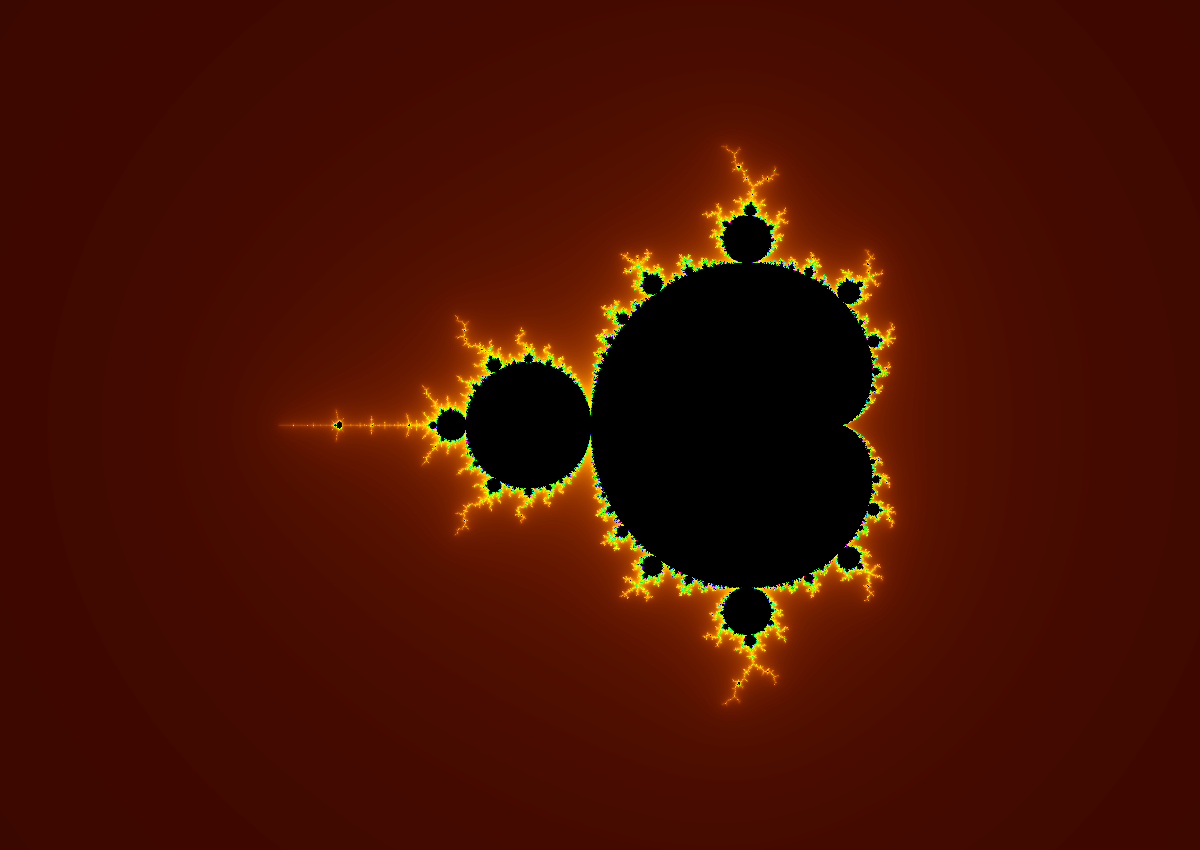
\includegraphics[width=\linewidth]{cover-fractal.png}
            \end{minipage}%
            \begin{minipage}[b]{0.02\textwidth}
                \hfill % Décalage horizontal
                \rotatebox[origin=rb]{90}{Photo: XEBX}
                \vspace*{\fill}
            \end{minipage}
        \end{figure}
        \vspace{0.5cm}
        {\huge \bfseries \titre} 
        \vfill
        {\huge \textbf{\auteur}} 
        \vfill
        {\Large \textbf{\dateTM} \\
        {\Large Domaine Ingénierie et Architecture} \\
        {\large Master conjoint UNIGE -- HES-SO en développement territorial} \\
        {\large Orientation \orientation}
        \vfill
        \small 
        Directeur : \directeur \\
        Co-directeur : \codirecteur \\
        Expert : \expert} 
        \vfill
        \small Mémoire no : \numeroTM 
    \end{flushleft}
    \vfill
    
\includegraphics[height=1.25cm]{unige.png}
    \hspace{1.5cm}
    
\includegraphics[height=1.25cm]{hesso.jpg}
    \vfill
\end{titlepage}

%%%% RESUME (FR) %%%%%
\cleardoublepage
\pagestyle{preliminary}
%%-----------------------------------------------------------------%%
%%
%%      Résumé/Description du Travail de Master en 1 page
%%
%%-----------------------------------------------------------------%%

\chapter*{Résumé}
\thispagestyle{empty}
\lipsum[1-4]

\vspace{1cm}
\underline{Mots-clés :} Photogrammétrie, GNSS, réseaux géodésiques, compensation par les moindres carrés, ...

%%%% RESUME (EN) %%%%%
\cleardoublepage
\pagestyle{preliminary}
%%-----------------------------------------------------------------%%
%%
%%      Résumé/Description du Travail de Master en 1 page
%%
%%-----------------------------------------------------------------%%

\chapter*{Summary}
\thispagestyle{empty}
\lipsum[1-4]

\vspace{1cm}
\underline{Keywords :} Photogrammétrie, GNSS, réseaux géodésiques, compensation par les moindres carrés, ...

%%%% Remerciement
\cleardoublepage
%%-----------------------------------------------------------------%%
%%
%%              Remerciements à certaines personnes
%%
%%-----------------------------------------------------------------%%

\chapter*{Remerciements}
\lipsum[1-2]
\thispagestyle{empty}

%%%% AVANT-PROPOS %%%%%
\cleardoublepage
%%-----------------------------------------------------------------%%
%%
%%  Preambule
%%  et pas avant-propos, source: https://www.edilivre.com/prologue-preambule-preface-introduction-comment-sy-retrouver/
%% Le préambule se rapproche de la préface à la différence qu’il est rédigé par l’auteur lui-même. 
%% Le préambule est un éclaircissement préliminaire plus ou moins utile, il donne un avant-goût de
%% l’ouvrage, en marque le caractère et la portée, ou résume les événements accomplis antérieurement
%% au récit. Le préambule doit être court et concis.
%%
%%-----------------------------------------------------------------%%

\chapter*{Préambule}
\thispagestyle{empty}
\lipsum[1-3]

%%%% TABLE DES MATIERES %%%%%
\clearemptydoublepage
\pagestyle{tablecontent}
\tableofcontents{}

%%%%% LISTE DES FIGURES %%%%%
\clearemptydoublepage
\listoffigures
\addcontentsline{toc}{chapter}{Liste des figures}

%%%%% LISTE TABLEAUX %%%%%
\clearemptydoublepage
\listoftables
\addcontentsline{toc}{chapter}{Liste des tableaux}

%%%%% LISTE DES EQUATIONS %%%%%

%%%%% LISTE D'ALGORITHMES %%%%%
\clearemptydoublepage
\lstlistoflistings
\addcontentsline{toc}{chapter}{\lstlistlistingname}

%%%%% ABBREVIATIONS %%%%%
\clearemptydoublepage
\glsaddallunused%            citer toutes les abréviations non utilisées
\printglossary[
    type=\acronymtype,%      afficher que les abbréviations
    title=Abréviations,%     titre du chapitre
    toctitle=Abréviations,%  titre du chapitre dans la table des matières
]

%%%%% CONSTANTS %%%%%
\clearemptydoublepage
\printnomenclature
\addcontentsline{toc}{chapter}{\nomname}

%%%%% INTRODUCTION %%%%%
\clearemptydoublepage
\pagestyle{fancy}
\chapter*{Introduction}
\addcontentsline{toc}{chapter}{Introduction}
\markboth{INTRODUCTION}{Introduction}

\section*{Contexte}
\section*{Cahier des charges}

%%%%% CHAPITRE %%%%%
\clearemptydoublepage
\chapter{Éléments théoriques}

\section{Introduction d'éléments théoriques}
Lorem ipsum dolor sit amet, consectetur adipiscing elit. Sed non risus. Suspendisse lectus tortor, dignissim sit amet, adipiscing nec, ultricies sed, dolor. Cras elementum ultrices diam. Maecenas ligula massa, varius a, semper congue, euismod non, mi. Proin porttitor, orci nec nonummy molestie, enim est eleifend mi, non fermentum diam nisl sit amet erat. Duis semper. Duis arcu massa, scelerisque vitae, consequat in, pretium a, enim. Pellentesque congue. Ut in risus volutpat libero pharetra tempor. Cras vestibulum bibendum augue. Praesent egestas leo in pede. Praesent blandit odio eu enim. Pellentesque sed dui ut augue blandit sodales. Vestibulum ante ipsum primis in faucibus orci luctus et ultrices posuere cubilia Curae; Aliquam nibh. Mauris ac mauris sed pede pellentesque fermentum. Maecenas adipiscing ante non diam sodales hendrerit.\\
Ut velit mauris, egestas sed, gravida nec, ornare ut, mi. Aenean ut orci vel massa suscipit pulvinar. Nulla sollicitudin. Fusce varius, ligula non tempus aliquam, nunc turpis ullamcorper nibh, in tempus sapien eros vitae ligula. Pellentesque rhoncus nunc et augue. Integer id felis. Curabitur aliquet pellentesque diam. Integer quis metus vitae elit lobortis egestas. Lorem ipsum dolor sit amet, consectetuer adipiscing elit. Morbi vel erat non mauris convallis vehicula. Nulla et sapien. Integer tortor tellus, aliquam faucibus, convallis id, congue eu, quam. Mauris ullamcorper felis vitae erat. Proin feugiat, augue non elementum posuere, metus purus iaculis lectus, et tristique ligula justo vitae magna.

\begin{center}
    \begin{longtable}{ll}
        \caption{Paramètres de calcul}\label{tab:Paramètres calcul tangent bruit saut}    \\
        \toprule
        Paramètre             & Valeur \tabularnewline
        \midrule
        \endhead
        Etat plateforme       & Statique et en mouvement\tabularnewline
        Date                  & 24.06.2020 \tabularnewline
        Début                 & UTC 14h 29min 24sec \tabularnewline
        Fin                   & UTC 14h 30min 15sec \tabularnewline
        Nb époques            & 51\tabularnewline
        Position approchée    & Positionnement absolu sur le code \tabularnewline
        Bruit                 & Oui (1m sur le code, 0.002 m sur la phase)\tabularnewline
        Sauts de cycles       & Oui \tabularnewline
        Quaternions approchés & Helmert 3D  \tabularnewline
        Estimation flottante  & Quaternions libérés, ambiguïtés libérées \tabularnewline
        Estimation fixe       & Quaternions libérés, ambiguïtés fixées \tabularnewline
        \bottomrule
    \end{longtable}
\end{center}

\begin{table}
    \begin{tabular}{c|c|c|c|c}
        \toprule
        Méthode                       & Absolu & Relatif & Observation  & Précision \\
        \midrule
        SPP Single Point Positioning  & x      &         & Code         & 5-10 m  \\
        PPP Precise Point Positioning & x      &         & Code + Phase & 0.05-0.20 m  \\
        Code différentiel             &        & x       & Code         & 0.5-1.0 m  \\
        Phase différentiel (\acrshort{rtk})      &        & x       & Phase        & 0.02 m + 2 ppm  \\
        \bottomrule
    \end{tabular}
    \caption{Méthodes de positionnement en temps réel}
    \label{tab:Positionnement temps réel} 
\end{table}

Aliquam convallis sollicitudin purus. Praesent aliquam, enim at fermentum mollis, ligula massa adipiscing nisl, ac euismod nibh nisl eu lectus. Fusce vulputate sem at sapien. Vivamus leo. Aliquam euismod libero eu enim. Nulla nec felis sed leo placerat imperdiet. Aenean suscipit nulla in justo. Suspendisse cursus rutrum augue. Nulla tincidunt tincidunt mi. Curabitur iaculis, lorem vel rhoncus faucibus, felis magna fermentum augue, et ultricies lacus lorem varius purus. Curabitur eu amet.

\begin{equation}
    f_r = f^s \cdot \left(\frac{1+ \left(\frac{\mathbf{e}\cdot v_r}{c}\right)}{1+ \left(\frac{\mathbf{e}\cdot v_s}{c}\right)}\right)
\end{equation}
\begin{equation}
    D_r^s = \frac{1}{\lambda} \cdot \left(\frac{\mathbf{v}^s}{c}-\mathbf{e}\right) \cdot (\mathbf{v}^s -\mathbf{v}_r) + ({df}_r - {df}^s) + \frac{c}{\lambda} \cdot \delta f_{clk}^{rel}
\end{equation}
Avec :
% [D_r^s] Mesure Doppler entre un satellite $s$ et un récepteur $r$ [Hz]
% [f_r] Fréquence de réception [Hz]
% [f^s] Fréquence d'émission [Hz]
% [c] Vitesse de la lumière dans le vide $\left[\frac{\text{m}}{\text{s}}\right]$
% [\mathbf{e}^i] Vecteur en direction du satellite depuis le récepteur
% [\lambda] Longueur d'onde du signal observé [m]
% [\mathbf{v}^s] Vecteur vitesse du satellite $\left[\frac{\text{m}}{\text{s}}\right]$
% [\mathbf{v}_r] Vecteur vitesse du récepteur $\left[\frac{\text{m}}{\text{s}}\right]$
% [{df}_r] Erreur de fréquence du récepteur [Hz]
% [{df}^s] Erreur de fréquence du satellite [Hz]
% [\delta f_{clk}^{rel}] Effets relativistes


\begin{equation}
    \boxed{
    P^{i}_{A} + {\hat{v}}_{P^{i}_{A}} = |\textbf{x}^i - {\hat{\textbf{x}}}_A| + c \cdot \hat{\delta t}^{rec_A}_{rec} - c \cdot {\delta t}^{sat_i}_{em} + \delta \rho^{i}_{A,trop} + \delta \rho^{i}_{A,iono}
    }
    \label{eq_obs_pseudodistance}
\end{equation}

\begin{equation}
    \mathbf{C} =
    \bordermatrix{
        & \hat{x_B}_1 & \hat{y_B}_1 & \hat{z_B}_1 & \hat{x_B}_2 & \hat{y_B}_2 & \hat{z_B}_2 & \ldots & \nabla \Delta \hat{N}^{ij}_{AB} & \nabla \Delta \hat{N}^{ik}_{AB} & \nabla \Delta \hat{N}^{il}_{AB} & \ldots & \nabla \Delta \hat{N^{iz}_{AB}}_n\cr
        \nabla \Delta \hat{N^{ij}_{AB}} & - & - & - & - & - & - & \ldots & 1 & - & - & - & -\cr
        \nabla \Delta \hat{N^{ik}_{AB}} & - & - & - & - & - & - & \ldots & - & 1 & - & - & -\cr
        \nabla \Delta \hat{N^{il}_{AB}} & - & - & - & - & - & - & \ldots & - & - & 1 & - & -\cr
        \vdots & - & - & - & - & - & - & \ddots & - & - & - & \ddots & - \cr
        \nabla \Delta \hat{N^{iz}_{AB}} & - & - & - & - & - & - & \ldots & - & - & - & - & 1\cr
    }
\end{equation}

Aliquam convallis sollicitudin purus. Praesent aliquam, enim at fermentum mollis, ligula massa adipiscing nisl, ac euismod nibh nisl eu lectus. Fusce vulputate sem at sapien. Vivamus leo. Aliquam euismod libero eu enim. Nulla nec felis sed leo placerat imperdiet. Aenean suscipit nulla in justo. Suspendisse cursus rutrum augue. Nulla tincidunt tincidunt mi. Curabitur iaculis, lorem vel rhoncus faucibus, felis magna fermentum augue, et ultricies lacus lorem varius purus. Curabitur eu amet.

\begin{figure}[ht]
    \begin{lstlisting}[language=Json]
    {
        "1680262162.9": {
            "gnss": {
                "timestamp": [
                    1680262162000.0,
                    1680262162100.0, 
                    1680262162900.0
                ],
                "longitude": [
                    6.656051646773433,
                    6.656051874781411,
                    6.656076635597395
                ],
                "latitude": [
                    46.77854614906064,
                    46.77854619764593,
                    46.77855147382547
                ],
                "altitude": [
                    435.8,
                    435.8,
                    435.8
                ]
            }
        },
    }
    \end{lstlisting}
    \caption{Structure de données des trajectoires}\label{fig:fichier_Json}
\end{figure}

Aliquam convallis sollicitudin purus. Praesent aliquam, enim at fermentum mollis, ligula massa adipiscing nisl, ac euismod nibh nisl eu lectus. Fusce vulputate sem at sapien. Vivamus leo. Aliquam euismod libero eu enim. Nulla nec felis sed leo placerat imperdiet. Aenean suscipit nulla in justo. Suspendisse cursus rutrum augue. Nulla tincidunt tincidunt mi. Curabitur iaculis, lorem vel rhoncus faucibus, felis magna fermentum augue, et ultricies lacus lorem varius purus. Curabitur eu amet.\\

\begin{lstlisting}[language=Python, caption=Exemple de fonction Python,captionpos=t]
import numpy as np
    
def incmatrix(genl1,genl2):
    m = len(genl1)
    n = len(genl2)
    M = None #to become the incidence matrix
    
    return M
\end{lstlisting}

\begin{center}
    \begin{figure}[ht]
        \centering
        \begin{tikzpicture}[node distance=3cm]
            \tikzstyle{etapes} = [rectangle, rounded corners,
            minimum width=1cm,
            minimum height=1cm,
            text centered,
            draw=black,
            fill=white!30]
            \definecolor{myblue}{RGB}{0, 0, 225}
            \tikzstyle{arrow} = [thick,->,>=stealth,myblue ]
            \node (etape1)[etapes]{WGS84};
            \node (etape2)[etapes, below of=etape1]{\begin{tabular}{c}\large WGS84 - ellipsoïdale\\ \large ($\mathbf{\lambda}^{\text{WGS84}}$,$\mathbf{\varphi}^{\text{WGS84}}$,$\mathit{h}^{\text{WGS84}}$)\end{tabular}};
            \node (etape3)[etapes, below of=etape2] {\begin{tabular}{c} \large UTM - altitude ellipsoïdale\\ \large($\mathit{E}^{\text{UTM}}$,$\mathit{N}^{\text{UTM}}$,$\mathit{h}^{\text{UTM}}$)\end{tabular}};
            \node (etape4)[etapes, below of=etape3] {\begin{tabular}{c} \large UTM-red\\ \large ($\mathit{E}^{\text{UTM-red}}$,$\mathit{N}^{\text{UTM-red}}$,$\mathit{h}^{\text{UTM-red}}$)\end{tabular}};
            \node (etape5)[etapes, below of=etape4] {\begin{tabular}{c}\large Unity\\ \large (x,y,z)\end{tabular}};

            \draw [arrow] (etape1) -- (etape2);
            \draw [arrow] (etape2) -- (etape3);
            \draw [arrow] (etape3) -- (etape4);
            \draw [arrow] (etape2) -- node[anchor=west,myblue] {\normalsize 1) Projection basée sur la
                projection de Mercator transverse ellipsoïdale} (etape3);
            \draw [arrow] (etape3) -- node[anchor=west,myblue] {\normalsize 2) 3 Translations} (etape4);
            \draw [arrow] (etape4) -- node[anchor=west,myblue] {\normalsize 3) Système de coordonnées main gauche } (etape5);
        \end{tikzpicture}
        \caption{WGS84 vers Unity}
    \end{figure}
\end{center}

Aliquam convallis sollicitudin purus. Praesent aliquam, enim at fermentum mollis, ligula massa adipiscing nisl, ac euismod nibh nisl eu lectus. Fusce vulputate sem at sapien. Vivamus leo. Aliquam euismod libero eu enim. Nulla nec felis sed leo placerat imperdiet. Aenean suscipit nulla in justo. Suspendisse cursus rutrum augue. Nulla tincidunt tincidunt mi. Curabitur iaculis, lorem vel rhoncus faucibus, felis magna fermentum augue, et ultricies lacus lorem varius purus. Curabitur eu amet. Aliquam convallis sollicitudin purus. Praesent aliquam, enim at fermentum mollis, ligula massa adipiscing nisl, ac euismod nibh nisl eu lectus. Fusce vulputate sem at sapien. Vivamus leo. Aliquam euismod libero eu enim. Nulla nec felis sed leo placerat imperdiet. Aenean suscipit nulla in justo. Suspendisse cursus rutrum augue. Nulla tincidunt tincidunt mi. Curabitur iaculis, lorem vel rhoncus faucibus, felis magna fermentum augue, et ultricies lacus lorem varius purus. Curabitur eu amet.

Aliquam convallis sollicitudin purus. Praesent aliquam, enim at fermentum mollis, ligula massa adipiscing nisl, ac euismod nibh nisl eu lectus. Fusce vulputate sem at sapien. Vivamus leo. Aliquam euismod libero eu enim. Nulla nec felis sed leo placerat imperdiet. Aenean suscipit nulla in justo. Suspendisse cursus rutrum augue. Nulla tincidunt tincidunt mi. Curabitur iaculis, lorem vel rhoncus faucibus, felis magna fermentum augue, et ultricies lacus lorem varius purus. Curabitur eu amet.

Aliquam convallis sollicitudin purus. Praesent aliquam, enim at fermentum mollis, ligula massa adipiscing nisl, ac euismod nibh nisl eu lectus. Fusce vulputate sem at sapien. Vivamus leo. Aliquam euismod libero eu enim. Nulla nec felis sed leo placerat imperdiet. Aenean suscipit nulla in justo. Suspendisse cursus rutrum augue. Nulla tincidunt tincidunt mi. Curabitur iaculis, lorem vel rhoncus faucibus, felis magna fermentum augue, et ultricies lacus lorem varius purus. Curabitur eu amet.

Aliquam convallis sollicitudin purus. Praesent aliquam, enim at fermentum mollis, ligula massa adipiscing nisl, ac euismod nibh nisl eu lectus. Fusce vulputate sem at sapien. Vivamus leo. Aliquam euismod libero eu enim. Nulla nec felis sed leo placerat imperdiet. Aenean suscipit nulla in justo. Suspendisse cursus rutrum augue. Nulla tincidunt tincidunt mi. Curabitur iaculis, lorem vel rhoncus faucibus, felis magna fermentum augue, et ultricies lacus lorem varius purus. Curabitur eu amet.

Aliquam convallis sollicitudin purus. Praesent aliquam, enim at fermentum mollis, ligula massa adipiscing nisl, ac euismod nibh nisl eu lectus. Fusce vulputate sem at sapien. Vivamus leo. Aliquam euismod libero eu enim. Nulla nec felis sed leo placerat imperdiet. Aenean suscipit nulla in justo. Suspendisse cursus rutrum augue. Nulla tincidunt tincidunt mi. Curabitur iaculis, lorem vel rhoncus faucibus, felis magna fermentum augue, et ultricies lacus lorem varius purus. Curabitur eu amet.

Aliquam convallis sollicitudin purus. Praesent aliquam, enim at fermentum mollis, ligula massa adipiscing nisl, ac euismod nibh nisl eu lectus. Fusce vulputate sem at sapien. Vivamus leo. Aliquam euismod libero eu enim. Nulla nec felis sed leo placerat imperdiet. Aenean suscipit nulla in justo. Suspendisse cursus rutrum augue. Nulla tincidunt tincidunt mi. Curabitur iaculis, lorem vel rhoncus faucibus, felis magna fermentum augue, et ultricies lacus lorem varius purus. Curabitur eu amet.

Aliquam convallis sollicitudin purus. Praesent aliquam, enim at fermentum mollis, ligula massa adipiscing nisl, ac euismod nibh nisl eu lectus. Fusce vulputate sem at sapien. Vivamus leo. Aliquam euismod libero eu enim. Nulla nec felis sed leo placerat imperdiet. Aenean suscipit nulla in justo. Suspendisse cursus rutrum augue. Nulla tincidunt tincidunt mi. Curabitur iaculis, lorem vel rhoncus faucibus, felis magna fermentum augue, et ultricies lacus lorem varius purus. Curabitur eu amet.

Aliquam convallis sollicitudin purus. Praesent aliquam, enim at fermentum mollis, ligula massa adipiscing nisl, ac euismod nibh nisl eu lectus. Fusce vulputate sem at sapien. Vivamus leo. Aliquam euismod libero eu enim. Nulla nec felis sed leo placerat imperdiet. Aenean suscipit nulla in justo. Suspendisse cursus rutrum augue. Nulla tincidunt tincidunt mi. Curabitur iaculis, lorem vel rhoncus faucibus, felis magna fermentum augue, et ultricies lacus lorem varius purus. Curabitur eu amet.

Aliquam convallis sollicitudin purus. Praesent aliquam, enim at fermentum mollis, ligula massa adipiscing nisl, ac euismod nibh nisl eu lectus. Fusce vulputate sem at sapien. Vivamus leo. Aliquam euismod libero eu enim. Nulla nec felis sed leo placerat imperdiet. Aenean suscipit nulla in justo. Suspendisse cursus rutrum augue. Nulla tincidunt tincidunt mi. Curabitur iaculis, lorem vel rhoncus faucibus, felis magna fermentum augue, et ultricies lacus lorem varius purus. Curabitur eu amet.

\section{Blabla quotidien}

Aliquam convallis sollicitudin purus. Praesent aliquam, enim at fermentum mollis, ligula massa adipiscing nisl, ac euismod nibh nisl eu lectus. Fusce vulputate sem at sapien. Vivamus leo. Aliquam euismod libero eu enim. Nulla nec felis sed leo placerat imperdiet. Aenean suscipit nulla in justo. Suspendisse cursus rutrum augue. Nulla tincidunt tincidunt mi. Curabitur iaculis, lorem vel rhoncus faucibus, felis magna fermentum augue, et ultricies lacus lorem varius purus. Curabitur eu amet.

\vspace{10pt}

Aliquam convallis sollicitudin purus. Praesent aliquam, enim at fermentum mollis, ligula massa adipiscing nisl, ac euismod nibh nisl eu lectus. Fusce vulputate sem at sapien. Vivamus leo. Aliquam euismod libero eu enim. Nulla nec felis sed leo placerat imperdiet. Aenean suscipit nulla in justo. Suspendisse cursus rutrum augue. Nulla tincidunt tincidunt mi. Curabitur iaculis, lorem vel rhoncus faucibus, felis magna fermentum augue, et ultricies lacus lorem varius purus. Curabitur eu amet.

Aliquam convallis sollicitudin purus. Praesent aliquam, enim at fermentum mollis, ligula massa adipiscing nisl, ac euismod nibh nisl eu lectus. Fusce vulputate sem at sapien. Vivamus leo. Aliquam euismod libero eu enim. Nulla nec felis sed leo placerat imperdiet. Aenean suscipit nulla in justo. Suspendisse cursus rutrum augue. Nulla tincidunt tincidunt mi. Curabitur iaculis, lorem vel rhoncus faucibus, felis magna fermentum augue, et ultricies lacus lorem varius purus. Curabitur eu amet.

Aliquam convallis sollicitudin purus. Praesent aliquam, enim at fermentum mollis, ligula massa adipiscing nisl, ac euismod nibh nisl eu lectus. Fusce vulputate sem at sapien. Vivamus leo. Aliquam euismod libero eu enim. Nulla nec felis sed leo placerat imperdiet. Aenean suscipit nulla in justo. Suspendisse cursus rutrum augue. Nulla tincidunt tincidunt mi. Curabitur iaculis, lorem vel rhoncus faucibus, felis magna fermentum augue, et ultricies lacus lorem varius purus. Curabitur eu amet.

Aliquam convallis sollicitudin purus. Praesent aliquam, enim at fermentum mollis, ligula massa adipiscing nisl, ac euismod nibh nisl eu lectus. Fusce vulputate sem at sapien. Vivamus leo. Aliquam euismod libero eu enim. Nulla nec felis sed leo placerat imperdiet. Aenean suscipit nulla in justo. Suspendisse cursus rutrum augue. Nulla tincidunt tincidunt mi. Curabitur iaculis, lorem vel rhoncus faucibus, felis magna fermentum augue, et ultricies lacus lorem varius purus. Curabitur eu amet.

Aliquam convallis sollicitudin purus. Praesent aliquam, enim at fermentum mollis, ligula massa adipiscing nisl, ac euismod nibh nisl eu lectus. Fusce vulputate sem at sapien. Vivamus leo. Aliquam euismod libero eu enim. Nulla nec felis sed leo placerat imperdiet. Aenean suscipit nulla in justo. Suspendisse cursus rutrum augue. Nulla tincidunt tincidunt mi. Curabitur iaculis, lorem vel rhoncus faucibus, felis magna fermentum augue, et ultricies lacus lorem varius purus. Curabitur eu amet.

Aliquam convallis sollicitudin purus. Praesent aliquam, enim at fermentum mollis, ligula massa adipiscing nisl, ac euismod nibh nisl eu lectus. Fusce vulputate sem at sapien. Vivamus leo. Aliquam euismod libero eu enim. Nulla nec felis sed leo placerat imperdiet. Aenean suscipit nulla in justo. Suspendisse cursus rutrum augue. Nulla tincidunt tincidunt mi. Curabitur iaculis, lorem vel rhoncus faucibus, felis magna fermentum augue, et ultricies lacus lorem varius purus. Curabitur eu amet.


\clearemptydoublepage
\chapter{Développement de l'application}
\section{Equations mathématiques}
Il est possible d'afficher des équations comme l'équation \ref{eq:newton} qui est la seconde loi de Newton :
\begin{equation} \label{eq:newton}
    F = m \cdot a 
\end{equation}

mais il est possible de légender une équation comme l'équation \ref{eq:pythagore} : 
\begin{equation}\label{eq:pythagore}
   c^2 = a^2 + b^2
\end{equation}

%%%%% CONCLUSION %%%%%
\clearemptydoublepage
\chapter*{Conclusion}
\addcontentsline{toc}{chapter}{Conclusion}
\lipsum[1]

%%%%% BIBLIOGRAPHIE %%%%%
\clearemptydoublepage
\nocite{*} % pour citer toutes les références présentes dans la bibliographie
\printbibliography[
    heading=bibintoc, % Pour afficher la bibliographie dans la table des matières
    %title={Références}
]


%%%%% ANNEXES
\clearemptydoublepage
\appendix
\addcontentsline{toc}{chapter}{Annexes}

\clearemptydoublepage
\chapter{Annexes informatiques}
Ce rapport est accompagné des annexes informatiques suivantes :
\begin{center}
    \begin{forest}
        for tree={
        font=\ttfamily,
        grow'=0,
        child anchor=west,
        parent anchor=south,
        anchor=west,
        calign=first,
        edge path={
                \noexpand\path [draw, \forestoption{edge}]
                (!u.south west) +(7.5pt,0) |- node[fill,inner sep=1.25pt] {} (.child anchor)\forestoption{edge label};
            },
        before typesetting nodes={
                if n=1
                    {insert before={[,phantom]}}
                    {}
            },
        fit=band,
        before computing xy={l=15pt},
        }
        [text1
            [text1.1
                    [text1.1.1]
                    [text1.1.2]
                    [text1.1.3]
            ]
            [text1.2
                    [text1.2.1]
                    [text1.2.2]
            ]
        ]
    \end{forest}
\end{center}

\end{document}
